这里我们讨论Weinberg第三章的散射理论。这里我们开始考虑粒子之间的相互作用。考虑粒子从无穷远到很近的地方发生相互作用然后再到无穷远。

\section{In and Out States}

\subsection{无相互作用多粒子态}
对于没有相互作用的多粒子态,我们可以认为是单粒子态的直积。那么对于一个有质量的多粒子态,我们进行Lorentz变换可以知道是:
\eq{\label{eq:multitrans}
    \begin{aligned}
        U(\Lambda,a)&\Psi_{_{p_{1},\sigma_{1},\eta_{1};p_{2},\sigma_{2},\eta_{2};\cdots}}=\exp\left(-ia_{\mu}(p_{1}^{\mu}+p_{2}^{\mu}+\cdots)\right)\\&\times\sqrt{\frac{(\overline{\Lambda}p_{1})^{0}(\overline{\Lambda}p_{2})^{0}\cdots}{p_{1}^{0}p_{2}^{0}\cdots}}\sum_{\sigma_{1}^{\prime}\sigma_{2}^{\prime}\cdots}D_{\sigma_{1}^{\prime}\sigma_{1}}^{(j_{1})}\left(W(\Lambda,p_{1})\right)D_{\sigma_{2}^{\prime}\sigma_{2}}^{(j_{2})}\left(W(\Lambda,p_{2})\right)\\&\times\Psi_{_{\Lambda p_{1},\sigma_{1}^{\prime},n_{1};\Lambda p_{2},\sigma_{2}^{\prime},n_{2};\cdots}}
    \end{aligned}
}
\rmk{注意,每一个单粒子$ i $ 我们有三个label:第一个是$ p_i $也就是能动量四矢量;第二个是$ \sigma_i $也就是Wigner Little Group的自由度;第三个是$ n_i $也就是这个粒子的种类。   }
复习一下其中$ W(\Lambda,p) $ 是Wigner Rotation,定义是:\cref{eq:Wignerrotation}也就是:$ W(\Lambda,p)=L^{-1}(\Lambda p)\Lambda L(p). $ 。其中D矩阵是SO(3)群的表示矩阵定义为:\cref{eq:Dtrans}。对于无质量的粒子是另一个表示就是$ \delta_{\sigma,\sigma'} exp(i \sigma \theta(\Lambda,p))$。同样的我们定义一个合理的normalization是:
\eq{
\begin{aligned}
&\left(\Psi_{p_{1}^{\prime},\sigma_{1}^{\prime},n_{1}^{\prime};\,
           p_{2}^{\prime},\sigma_{2}^{\prime},n_{2}^{\prime};\cdots},
       \Psi_{p_{1},\sigma_{1},n_{1};\,
           p_{2},\sigma_{2},n_{2};\cdots}\right) \\
&= \delta^3(\mathbf{p}_1^{\prime}-\mathbf{p}_1)
   \delta_{\sigma_1^{\prime}\sigma_1}
   \delta_{n_1^{\prime}n_1}
   \delta^3(\mathbf{p}_2^{\prime}-\mathbf{p}_2)
   \delta_{\sigma_2^{\prime}\sigma_2}
   \delta_{n_2^{\prime}n_2}
   \cdots \\
&\quad \pm\ \text{permutations}
\end{aligned}
} 
这里面考虑了所有permutation的情况。但是注意,会有$ \pm $是因为会有bosonic的情况以及fermionic的情况。
\rmk{我们注意,上面的delta函数都是动量空间三维的。因为我们考虑的都是【同一质量的粒子对应的量子态】。我们不考虑不同质量的粒子量子态的内积。结果是delta函数也很合理,毕竟所有Hermite算符不同本征值的本征函数是正交的。但是系数是1是因为我们取了一个特殊normalization。这个内容具体请复习\cref{sec:normalization}}
\imp{多粒子态简洁记号}{
    为了进行简洁的书写多粒子态我们一般用这样的一个记号来表示:
\eq{
    (\Psi_{\alpha^{\prime}},\Psi_\alpha)=\delta(\alpha^{\prime}-\alpha)
}
注意这里$ \delta(\alpha^{\prime}-\alpha) $ 是一个记号并不是delta函数。并且积分我们也可以这么写:
\eq{
    \int d\alpha\cdots\equiv\sum_{n_{1}\sigma_{1}n_{2}\sigma_{2}\cdots}\int d^{3}p_{1}d^{3}p_{2}\cdots.
}
所以上面的内积结果completeness equation可以写作:
\eq{
    \Psi=\int d\alpha\Psi_\alpha(\Psi_\alpha,\Psi).
}
}
\rmk{注意,我们之前讨论的无相互作用的多粒子态,我们使用的是能动量四矢量+自旋or helicity进行标记说明\hlr{我们考虑满足这个变换的量子态一定是能动量的本征态。}}
我们考虑一个特殊的时间平移Lorentz变换也就是$ \tensor{\Lambda}{^\mu_\nu} = \delta^\mu_\nu $以及$ a^\mu = (0,0,0,\tau) $。在这个情况下我们的能量可以根据\cref{eq:multitrans}写成:
\eq{
    H\Psi_\alpha=E_\alpha\Psi_\alpha
}
其中$ E_\alpha = p^0_1+p^0_2+... $ 。


\subsection{In and Out States定义}

\hlr{现在我们不考虑无相互作用的粒子,而是考虑一个有相互作用的散射过程。}但是这个过程有个特点,就是在我们认为在$ - \infty $以及$ +\infty $的时间,粒子相当于没有相互作用的。  

\imp{In and Out的基本思路}{
    描述散射过程我们需要考虑结果和初始。这两个阶段粒子都应该没有相互作用了,并且时间是$ - \infty $以及$ +\infty $的点。
    
    所以对于散射过程我们可以定义两个量子态$  \Psi_\alpha^+, \Psi_\alpha^- $我们希望这两个量子态表征散射的初始状态和结果状态。所以我们赋予要求:
    \itm{
        \pt{这两个量子态对于「在$ \pm\infty $ 时间的观察者来说,等价于$ \Psi_\alpha $的量子态 」}
    }
}
\rmk{
    我们进行三个解读:
    \itm{
        \pt{首先,我们一直使用的是Heisenberg Picture进行描述量子态。\hlr{我们不认为量子态是定义在一个等时面的。而是描述整个时空全部的。量子态是与时间空间无关的向量。}但是我们知道不同观察者观察到的同一个量子态,但是观测到的是不同Hilbert空间上的矢量。}
    }

    一个具体的例子,考虑一个观察者B,他在A的未来时刻$ t_B = t_A - \tau $【注意这里的符号】。当一个事件在A的时间$ t_A = \tau $ 发生的时候,对于B来说这个时间就在$ t_B = 0 $发生。
    
    对于未来的观察者来说,如果A观察者在某一个时刻观察到了一个量子态$ \Psi_\alpha $,那么对于B来说,他在这个事件发生同时观测到的量子态就是$ U(Id,-\tau) \Psi_\alpha = e^{-iH\tau} \Psi$ 。

    这也就是时间平移算符的正负号的来源,请注意。
}
\rmk{\itm{
    \pt{第二个值得注意的是,我们既然如此,并不存在绝对的量子态,而是存在不同时间的量子态的相对关系,除非我们定义一个时间点。}
}
但是,这里我们知道不论定义哪个时间点。我们对于负无穷时间的观察者,如果时间发生在自己的时间0点(当然选哪个有限的时间都是一样的。)那么一般的观察者会知道这个事件发生在$ -\infty $的时间点。对于正无穷时间的观察者来说,他会知道这个事件发生在$ +\infty $的时间点。所以$ t_{\mp\infty} = t_A -(\mp \infty) $。这个才是正确的洛伦兹变换,以及怎么理解这件事。 

这个操作只有对in and out states这样的无穷时间的态才能这么定义,对于有限时间的态我们还是需要定义什么样的观察者看到的就是这样的态。\YL{这个是我自己的理解我觉得并不一定正确。我觉得需要讨论一下。}
}
\rmk{   

\itm{
    \pt{还有值得注意的是:什么叫"在$ \infty $时间等价于无相互作用粒子态"。因为我们考虑的量子态都是能动量本征态,那么由于不确定性原理,这样的量子态必然是弥散在时间和空间上面的。}
}

从数学的角度,如果我们直接对于$ \Psi_\alpha $量子态进行时间演化。我们会得到的$  U(Id,-\tau) = e^{-iH\tau}= e^{-E_\alpha \tau} $就是一个相位。是没有意义的,因为相差相位的量子态是同一个量子态。

所以我们需要额外技术解决这个问题。我们将考虑“\hlr{在波包的意义下},量子态在$ \infty $时间等价于无相互作用粒子”。具体写出来就是,我们定义一个波包的superposition的系数是$ g(\alpha) $并要求这个相位满足:【连续的叠加一些在有限范围$ \Delta E $的量子态 】
在这个的基础上我们可以定义设么叫:【在$ \infty $时间等价于无相互作用粒子态 】公式表达是:
\eq{
    \exp(-iH\tau)\int d\alpha\mathrm{~g}(\alpha)\Psi_\alpha^\pm=\int d\alpha\mathrm{~e}^{-iE_\alpha\tau}g(\alpha)\Psi_\alpha^\pm
}
分别对于$ \tau \gg 1/\Delta E $ 和$ \tau $远小于$ -1/\Delta E $
\YL{【不知道为啥,但是远小于符号就是打不出来!!】}
}

在上面充分的讨论的基础上我们就可以严格的定义in and out states了。

\imp{In and Out states严格定义}{
    我们研究一个散射过程之中我们使用的Hamiltonian可以写作下面的形式:
    \eq{
        H = H_0 + V
    }
    其中$ H_0 $代表没有相互作用的部分,而$ V $代表粒子之间的相互作用。并且我们要求:
    \itm{
        \pt{$ H $和$ H_0 $ 必须有一模一样的spectrum。也就是两个Hamiltonian的本征值是一样的。 }
    }
    这个要求本质上就是要求$ H_0 $并不是单纯的$ H $把所有的势能项直接删掉,我们需要定义一个新的质量,保证新的质量定义之下$ H_0 $ 的spectrum和之前的一样。为了定义新的质量减去的一些term要放到V里面去。  
    
    \defi{
      无相互作用多粒子态

      无相互作用的多粒子处于无相互作用的Hamiltonian也就是$ H_0 $ 的本征态,$ \Phi_\alpha $满足:
      \eq{
        H_0\Phi_x=E_x\Phi_x,\quad (\Phi_{x^{\prime}},\Phi_x)=\delta(\alpha^{\prime}-\alpha).
      } 
    }

    由于两个Hamiltonian有一样的spectrum所以我们下面可以定义In and Out state:
\defi{
  in and out states定义

  in and out states是满足下面两个条件的量子态:
 \begin{enumerate}
        \item 【对于$ H $来说 】和$ \Phi_\alpha $ 对于$ H_0 $来说有一样本征值的量子态$ \Phi_{\alpha}^{\pm} $也就是说:
        \eq{
            H\Psi_\alpha^\pm=E_\alpha\Psi_\alpha^\pm
        }
        \item 在$ \infty $等价于$ \Phi_\alpha $态:
        \eq{\label{eq:secondconditiontofreepartical}
            \int d\alpha\mathrm{~}e^{-iE_{x}\tau}g(\alpha)\Psi_{\alpha}^{\pm}\to\int d\alpha\mathrm{~}e^{-iE_{x}\tau}g(\alpha)\Phi_{\alpha}
        }
        分别对于$ \tau \to \mp \infty $。注意$ \Psi^+_\alpha $是in state对应的是$ \tau = -\infty $ 。

    \end{enumerate}

}
        对于这个关系我们有一个形式化的算符表达:
        \eq{
            \exp(-iH\tau)\int d\alpha\mathrm{~g}(\alpha)\Psi_\alpha^\pm\to\exp(-iH_0\tau)\int d\alpha\mathrm{~g}(\alpha)\Phi_\alpha
        }
        这个式子我们可以写成:
        \eq{\label{eq:timeinoutstate}
            \Psi_{\alpha}{}^{\pm}=\Omega(\mp\infty)\Phi_{\alpha},
        }
        其中我们定义:
        \eq{
            \Omega(\tau)\equiv\exp(+iH\tau)\exp(-iH_0\tau).
        }
        注意这个仅仅是一个形式化的表达。等式\cref{eq:timeinoutstate}是在「考虑波包」的意义下成立的。
}

\subsection{In and Out states的性质}
下面我们讨论这样的in and out states满足什么样的性质:
\bigskip

\hlr{性质1: in and out states是互相正交归一的量子态}

我们考虑in和in states或者out 和 out states之间的内积,我们会发现根据\cref{eq:secondconditiontofreepartical}存在in and out states的内积和自由多粒子态的内积之间的关系:
\eq{
    \int d\alpha d\beta\exp(-i(E_\alpha-E_\beta)\tau)g(\alpha)g^*(\beta)(\Psi_\beta^\pm,\Psi_\alpha^\pm)=\\
\int d\alpha d\beta\exp(-i(E_\alpha-E_\beta)\tau)g(\alpha)g^*(\beta)(\Phi_\beta,\Phi_\alpha).
}
由于这个关系对于所有任取的波包 $ g(\alpha) $都成立,所以我们立刻知道只有当满足:
\eq{
    (\Psi_\beta^\pm,\Psi_\alpha^\pm)=(\Phi_\beta,\Phi_\alpha)=\delta(\beta-\alpha).
}
这就说明in and out states是正交的。各自是一组Hilbert空间的正交归一基,就和自由例子态一样的!!
\rmk{
注意正交和完备性是两个概念,正交的定义是$ \braket{a_i}{a_j}= \delta_{ij} $;而完备的定义是$ \sum_i \ket{a_i}\bra{a_i} = 1 $ 。 

物理之中,我们一般认为我们的这些基是完备的。虽然我们并不能证明。但是这些基是有实际的物理意义的,就是具体的粒子。我们认为世界上只存在这样的粒子,所以就是完备的。}
\rmk{我们注意,这个是in和in state或者 out和out state之间内积的结果。我们不考虑in和out state之间的内积。}

\hlr{性质2: in and out states的explicit形式}

其实满足定义的两条关系我们可以形式化的写出一个explicit的形式。我们首先把定义之中的$ H = H_0+V $进行展开:
\eq{\label{eq:formalrewriteinout}
    (E_\alpha-H_0)\Psi_\alpha^\pm=V\Psi_\alpha^\pm.
} 
然后我们意识到,由于$ \Phi_\alpha $ 也是本征值为$ H_\alpha $但是是$ H_0 $ 的本征态,所以我们有:$( E_\alpha-H_0 )\Phi_\alpha = 0 $也就是算符$ ( E_\alpha-H_0 ) $ 湮灭了$ \Phi_\alpha $量子态。于是\cref{eq:formalrewriteinout}可以写作:
\eq{\label{eq:perturbannilationabit}
    (E_\alpha-H_0)(\Psi_\alpha^\pm-\Phi_\alpha)=V\Psi_\alpha^\pm.
}
这个时候我们希望把两边乘以算符$ (E_\alpha-H_0) $的逆。但问题是这个算符并不可逆,因为它的零空间并不是0,存在$ \Phi_\alpha $在零空间里。所以我们使用一个小技巧,我们把这个算符稍微perturb一下,我们考虑下面的算符:   
\eq{
    (E_\alpha-H_0 \pm i\epsilon)
}
我们规定研究in states的时候$ +i\epsilon $研究out states的时候$ -i\epsilon $。在这个基础上我们可以形式化写出来$ \Psi_\alpha $满足的一个形式:
\eq{\label{eq:preLSequation}
    \Psi_{\alpha}^{\pm}=\Phi_{\alpha}+(E_{\alpha}-H_{0}\pm i\epsilon)^{-1}V\Psi_{\alpha}^{\pm},
}   
\rmk{但是显然,这个形式并不是唯一的,因为$ (E_\alpha-H_0) $算符湮灭的可能不仅仅有$ \Phi_\alpha $一个量子态,可能有多重简并的;除此之外公式\cref{eq:perturbannilationabit}里面我们显然减去所有煎饼果子的态,减去任意多个都是成立的,所以形式并不唯一。 

考虑到上面的remark我们下面给出说明,只有写成这样的形式我们才能搞出满足第二个条件而且物理上看起来合理的in and out states的explicit形式。
}
在这些讨论的基础上我们给出:
\imp{Lippmann-Schwinger Equation}{
    这个方程给出了in and out states的explicit形式,我们对于\cref{eq:preLSequation}的右边的$ V\Psi_{\alpha}^{\pm} $量子态对于一个正交完备基进行展开,我们使用自由多粒子态作为正交完备基,结论是:
    \eq{\label{eq:LSequation}
        \begin{aligned}\Psi_{\alpha}^{\pm}&=\Phi_{\alpha}+\int d\beta\frac{T_{\beta\alpha}^{\pm}\Phi_{\beta}}{E_{\alpha}-E_{\beta}^{\pm}i\epsilon},\\T_{\beta\alpha}^{\pm}&\equiv(\Phi_{\beta},V\Psi_{\alpha}^{\pm}),\end{aligned}
    } 
    这个就是具体的形式。
}
下面我们验证这个方程给出的in and out states的具体形式,第二个性质就是相当于我们考虑下面两个量之间的差值是否在$ \tau \to \infty $的时候趋近于0:
\eq{\label{eq:definegt}
    \Psi_g^\pm(t)\equiv\int d\alpha e^{-iE_xt}g(\alpha)\Psi_x^\pm,\\\Phi_g(t)\equiv\int d\alpha e^{-iE_xt}g(\alpha)\Phi_\alpha.
} 
根据公式:\cref{eq:LSequation} 我们知道这两个量的差值就是:
\eq{\label{eq:differenceofLS}
    \int d\alpha e^{-iE_xt}g(\alpha)\Psi_x^\pm-\int d\alpha e^{-iE_xt}g(\alpha)\Phi_\alpha = \int d\alpha\int d\beta\frac{e^{-iE_{\alpha}t}g(\alpha)T_{\beta\alpha}{}^{\pm}\Phi_{\beta}}{E_{\alpha}-E_{\beta}\pm i\epsilon}.
}
也就是我们需要研究积分:
\eq{\label{eq:integralofLS}
    \int d\alpha\int d\beta\frac{e^{-iE_{\alpha}t}g(\alpha)T_{\beta\alpha}{}^{\pm}\Phi_{\beta}}{E_{\alpha}-E_{\beta}\pm i\epsilon}.
}
在$ t \to 0 $的取值结果。
\rmk{我们回忆积分是什么意思,是:\hlr{对于所有【三维的动量】进行积分,对于所有自旋以及粒子种类进行求和。}

我们对于三维空间的动量进行积分,因为确定粒子的质量之后,动量的自由度其实只有三维,能量等于$ \sqrt{p^2-M^2}  $。 
} 
对于离散的求和我们没有什么好说的,我们先对其确定自旋和粒子种类,对于所有粒子的三维空间的动量进行积分。对于积分\cref{eq:integralofLS}我们首先进行积分变量互换,先积分$ \alpha $的部分 :
\eq{
    \mathscr{F}_{\beta}{}^{\pm}\equiv\int d\alpha\frac{e^{-iE_{\alpha}t}g(\alpha)T_{\beta\alpha}{}^{\pm}}{E_{\alpha}-E_{\beta}\pm i\epsilon}.
}
\hlr{我们先考虑in states的情况,也就是取+的情况}

动量的积分是对于整个实轴进行积分。但是我们发现这个积分等于一个特殊的围道积分,如下图:
\begin{figure}[H]
    \centering
    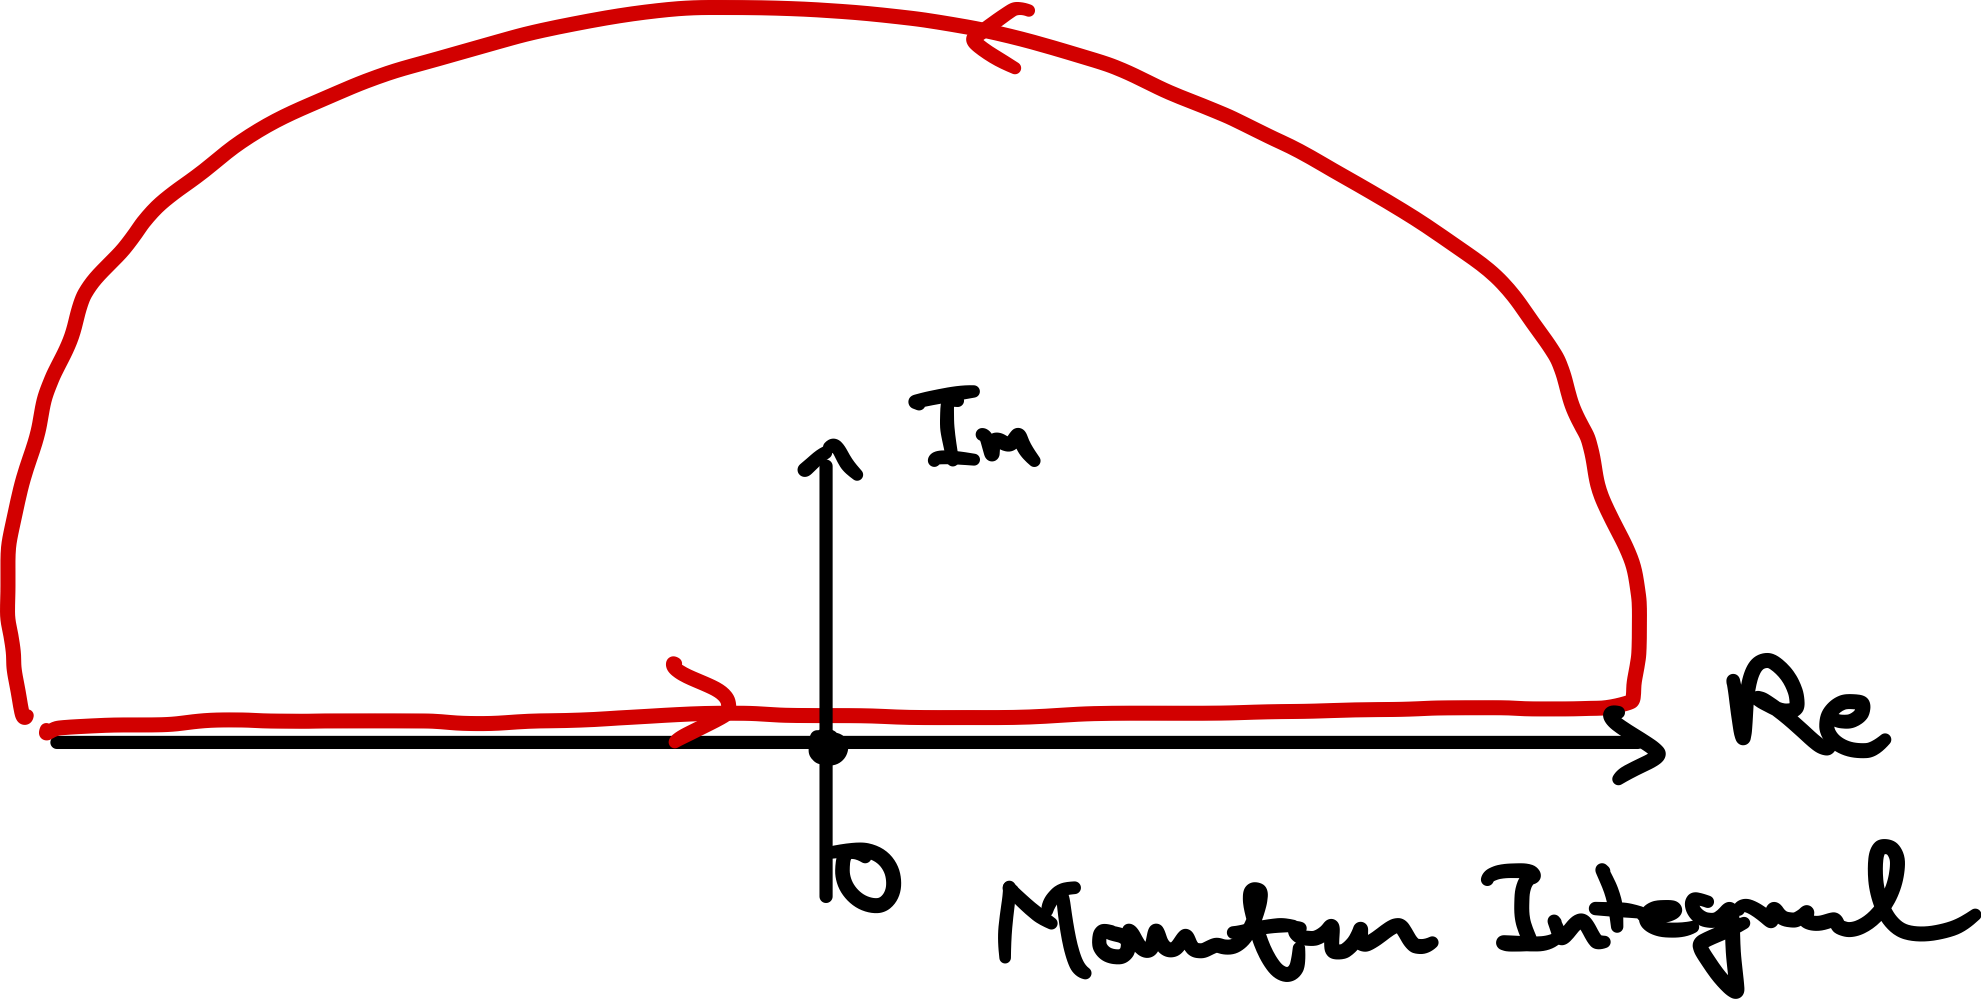
\includegraphics[width=0.4\textwidth]{2025-07-21-14-05-54.png}
    \caption{积分曲线}
    \label{fig:inteloop}
\end{figure}
对于in state,我们的$ t \to -\infty $。对于复平面的动量来说,由于是上半平面,$ p = p_{Re} +\mathrm{i}p_{Im}$并且$ p_{Im} >0 $。所以,由于$ \sqrt{p^2-M^2} = E_\alpha  $ 所以$ E_\alpha = E_{Re} +\mathrm{i}E_{Im} $ 并且$ E_{Im}>0 $。因此:
\eq{
    e^{-iE_\alpha t} = e^{-iE_{Re}t}e^{E_{Im}t} 
} 
当$ t \to -\infty $的时候,$ e^{E_{Im}t} \to 0 $。所以我们可以把围道积分的上半平面部分的积分结果是0。

下面,我们考虑这个围道里面的极点。我们注意到极点是$ E_\alpha = E_\beta -i\epsilon $并不在围道里面,所以并没有留数,所以积分是0。

\YL{[我有两个问题:1.到底为什么认为分子是没有极点的。2.似乎取$ +\mathrm{i}\epsilon $是纯粹恰好取的,这似乎就是凑出来的呃呃呃呃。]}

\hlr{然后考虑out states的情况}
会发现同样的,但是我们在下半平面进行围道积分,结果依旧是0.

综上,我们的\cref{eq:differenceofLS}等式右面是0。所以可以证明我们的LS方程确实表征了in and out states的explicit形式。

\subsection{一个特殊记号}

我们在LS方程之中使用了$ (E \pm \mathrm{i} \epsilon)^{-1} $这个算符。这个算符有一个改写方法:
\eq{
    (E\pm i\epsilon)^{-1}=\frac{\mathscr{P}_\epsilon}{E}\mp i\pi\delta_\epsilon(E),
} 
其中涉及的两个函数是:
\eq{
    \frac{\mathscr{P}_\epsilon}{E}\equiv\frac{E}{E^2+\epsilon^2},\quad \delta_\epsilon(E)\equiv\frac{\epsilon}{\pi(E^2+\epsilon^2)}.
}
我们分别讨论两个函数:
\itm{
    \pt{对于$ \frac{\mathscr{P}_\epsilon}{E} $我们会发现当$ E \gg \epsilon $的时候就是$ 1/E $但是在0附近就变成了0.所以相当于给了$ 1/E $一个在实轴上面积分的可能,把发散去除了。}
    \pt{$ \delta_\epsilon(E) $则类似delta函数,把0点附近的发散补了回来,但是是以delta函数的方式。 }
}

\section{S-matrix}
我们定义了in and out states之后我们可以使用一个振幅来表征从某一个in state经过散射到达某一个out state的概率,这个振幅我们定义为S-matrix。

\imp{S-matrix定义}{
    我们定义矩阵也就是一个in state和一个out state之间的内积为:
    \eq{
        S_{\beta x}=(\Psi_{\beta}^{-},\Psi_{\alpha}^{+}).
    }
}
我们下面讨论这个矩阵的一些性质:
\bigskip

\hlr{1. }如果没有相互作用V,那么in and out states就是完全一样的所以 $ S_{\alpha\beta} = \delta(\alpha-\beta) $ 所以我们可以用S矩阵和delta函数的区别表征一个反应的概率。

\rmk{in and out states是生活在同样的一个Hilbert空间之中的两个量子态,他们只是label的定义方式不一样,一个是趋近于正无穷定义的;另一个是趋近于负无穷。}
\bigskip

\hlr{2.} S矩阵是unitary的。也就是$ S^\dagger S = 1 $。

因为S矩阵相当于某一个Hilbert空间的两组正交基的变换矩阵,显然应该是Unitary的矩阵。同时,我们可以根据定义有:
\eq{
    \int d\beta S_{\beta\gamma}^*S_{\beta\alpha}=\int d\beta(\Psi_\gamma^+,\Psi_\beta^-)(\Psi_\beta^-,\Psi_\alpha^+)=(\Psi_\gamma^+,\Psi_\alpha^+).
}
中间第二步使用了完备的条件,我们并没有证明这是完备的,但是我们相信,对于我们考虑的物理世界,in and out states都是完备的基。最后根据正交性条件我们有:
\eq{
    \int d\beta S_{\beta\gamma}^{*}S_{\beta\alpha}=\delta(\gamma-\alpha)
}
同理有:
\eq{
    \int d\beta\mathrm{~}S_{\gamma\beta}S_{\alpha\beta}^*=\delta(\gamma-x)
}
所以我们的S矩阵是Unitary的矩阵。
\bigskip

\hlr{3.} S矩阵的另一个定义。我们有的时候会通过一个算符S和自由粒子态定义S矩阵。
\imp{S矩阵等价定义}{
    我们之前定义自由粒子态是$ \Phi_\alpha $ 那么S矩阵可以写成这样的形式:
    \eq{
        (\Phi_{\beta},S\Phi_{\alpha})\equiv S_{\beta\alpha}.
    }
我们考虑写作这个形式的S算符是什么,我们回顾形式化的表达:\cref{eq:timeinoutstate}。所以我们知道可以使用$ \Omega $算符来表达S算符:
\eq{
    S=\Omega(\infty)^{\dagger}\Omega(-\infty)=U(+\infty,-\infty)\mathrm{~,}
} 
其中我们还可以定义:
\eq{
    U(\tau,\tau_0)\equiv\Omega(\tau)^\dagger\Omega(\tau_0)=\exp(iH_0\tau)\exp(-iH(\tau-\tau_0))\exp(-iH_0\tau_0).
}
}   
\rmk{注意我们的$ \Omega $算符只是形式化表达,只用作用下一个小波包上面才有意义。}

\hlr{4. }我们下面意识到S矩阵还有一个explicit的表达方式。当我们参考使用LS方程的积分形式,我们考虑对于一个in states都是完备的基。最后根据正交性条件我们有\cref{eq:differenceofLS}也就是:
\eq{\label{eq:phipsirelation}
    \Psi_\mathrm{g}^+(t)=\Phi_\mathrm{g}(t)+\int d\alpha\int d\beta\frac{e^{-iE_\alpha t}g(\alpha)T_{\beta\alpha}{}^+\Phi_\beta}{E_\alpha-E_\beta+ i\epsilon}.
}
但是我们计算后面的项的时候我们强行取$ t \to +\infty $,所以应该在下半平面进行积分。这个和out state不同因为out state分母上面是:$ E_\alpha-E_\beta- i\epsilon $ 所以我们在下半平面没有极点。但是对于$ E_\alpha-E_\beta+ i\epsilon $来说我们选择下半平面进行积分之后存在极点以及不为0的留数。

「注意,我们围道积分是顺时针的,所以积分结果是$ -2 \pi \mathrm{i} $ 的留数」

我们依旧考虑这个积分的结果是什么:
\eq{
     \mathscr{F}_{\beta}{}^{+} = \int d\alpha\frac{e^{-iE_{\alpha}t}g(\alpha)T_{\beta\alpha}{}^{+}}{E_{\alpha}-E_{\beta}\pm i\epsilon}.
}
我们知道留数出现在$ \epsilon $趋于0的时候基本上就是$ E_\alpha = E_\beta $的时候。所以,我们可以把积分结果写作:
\eq{
    \mathscr{F}_{\beta}{}^+(t \to \infty )\to-2i\pi e^{-iE_{\beta}t}\int dx\delta(E_{\alpha}-E_{\beta})g(\alpha){T_{\beta\alpha}}^{+}
}  
写开之后我们带入之前的\cref{eq:phipsirelation}可以展开写成,对于$ t \to +\infty $的情况下,我们有 :
\eq{\label{eq:integraldeduction}
    \Psi_g^+(t\to \infty)\to\int d\beta e^{-iE_\beta t}\Phi_\beta\left[g(\beta)-2i\pi\int d\alpha\delta(E_\alpha-E_\beta)g(\alpha)T_{\beta\alpha}^+\right].
}
\line
同时我们知道,使用S矩阵可以把$ \Psi_\alpha^{+} $使用$ \Psi_\beta^{-} $进行展开展开结果是:
\eq{
   \Psi_\alpha^{+} =  \int d\beta\Psi_{\beta}^-S_{\beta\alpha}.
} 
我们把这个带入到$ \Psi_g^+(t) $的定义\cref{eq:definegt}得到的结果是:
 \eq{
    \Psi_g^+(t)=\int dxe^{-iE_\alpha t}g(\alpha)\int d\beta\Psi_\beta^-S_{\beta\alpha}.
 }
由于我们认为$ S_{\alpha\beta} $矩阵之中包含一个$ \delta(\alpha - \beta) $的样子,所以我们不妨改变积分顺序并把$ \Psi_\beta^- $提到对$ \alpha $积分的前面。\YL{我对于这个操作是否合法深表怀疑,关于S矩阵能够代表delta函数我很怀疑对于一般情况这个是否成立。}但总之我们写作:
\eq{
    \Psi_{g}^{+}(t)=\int d\beta\Psi_{\beta}^{-}e^{-iE_{\beta}t}\int d\alpha g(\alpha)S_{\beta\alpha}
}
我们考虑这个式子$ t \to \infty $的极限,由于在无穷极限下面$ \Psi $逐渐类似于$ \Phi $\YL{这也是一个禁不起考验的论断呃呃,似乎就是物理直观并不严谨。}我们有:
\eq{\label{eq:Smatrixdudction}
    \Psi_g^+(t)\to\int d\beta\Phi_\beta e^{-iE_\beta t}\int d\alpha g(\alpha)S_{\beta\alpha}.
}   

最终我们对比\cref{eq:Smatrixdudction}以及\cref{eq:integraldeduction}这个两个不同的推导过程导出的$ t \to \infty $呃情况下$ \Psi_g^+(t) $  的结果。我们有:
\eq{
    \int d\alpha\mathrm{~g}(\alpha)S_{\beta\alpha}=\mathrm{g}(\beta)-2\mathrm{i}\pi\int d\alpha\mathrm{~}\delta(E_\alpha-E_\beta)\mathrm{g}(\alpha)T_{\beta\alpha}{}^+
}
对于这个结果我们意识到了一个S矩阵的explicit的表达式:
\eq{
    S_{\beta\alpha}=\delta(\beta-\alpha)-2i\pi\delta(E_{\alpha}-E_{\beta}){T_{\beta\alpha}}^{+}
}
\imp{Born Approximation}{
    当相互作用V比较小的时候,我们可以忽略in state和free particle的区别于是得到近似:
    \eq{
        S_{\beta\alpha}\simeq\delta(\beta-\alpha)-2i\pi\delta(E_{\alpha}-E_{\beta})(\Phi_{\beta},V\Phi_{\alpha})\mathrm{~.}
    }
}
